

\section{Graphs}
Graphs encode the idea of connections between things, for example
\begin{itemize}
\item networks of computers
\item people and their relationships
\item cities and highways
\item sets and intersections
\item workers and tasks
\end{itemize}


In formal mathematical terms, a graph is:
\begin{defn}
A \Xb{graph} $G$ is an ordered triple $(V, E, \psi)$ consisting of
\begin{itemize}
\item a finite, nonempty set $V$, whose elements are referred to as vertices,
\item a finite (possibly empty) set $E$, whose elements are referred to as
edges, and
\item an ``incidence'' function $\psi: E \to \ms R_2(V)$,
\end{itemize}
where $\ms R_2(V)$ is the set of unordered pairs of elements of $V$ (which
one may also think of as two elements multisubsets of $V$ -- see
Definition~\ref{multisubsets definition}).
\end{defn}

We represent such graphs visually by drawing vertices as dots or circles,
and edges as lines between them. For example, the drawing in
Figure~\ref{basic graph} would stand for the graph $G$ defined by $V_G =
\{A, B, C, D\}, E_G = \{1, 2, 3, 4, 5\}$ and incidence function $\psi_G$
given by:
\[\psi_G(1) = AC, \ \psi_G(2) = BC, \ \psi_G(3) = CD, \ \psi_G(4) = AD, \
\psi_G(5) = BD.\]

\begin{figure} \label{basic graph}
\caption{}
\begin{center}
\begin{tikzpicture}[scale=0.75,transform shape]
  \Vertex[x=0,y=0]{A}
  \Vertex[x=3,y=3]{B}
  \Vertex[x=0,y=3]{C}
  \Vertex[x=3,y=0]{D}

  \tikzstyle{LabelStyle}=[fill=white]

  \Edge[label=$1$](A)(C)
  \Edge[label=$2$](B)(C)
  \Edge[label=$3$](C)(D)
  \Edge[label=$4$](D)(A)
  \Edge[label=$5$](B)(D)
\end{tikzpicture}
\end{center}
\end{figure}

\begin{notn}
For a graph $G = (V, E, \psi)$ we write $V_G$ for $V$, $E_G$ for $E$ and
$\psi_G$ for $\psi$.
\end{notn}
In other words, using this notational convention, if we are given graphs
$G, H, K$, and have not specified letters for their sets of vertices,
edges, etcetera, we may write, for example, $E_K$ for the edges of the
graph $K$, $V_H$ for the vertices of $H$, and $\psi_G$ for the incidence
function of $G$.

\begin{defn} \label{def:trivial}
A graph is called \textbf{trivial}\index{graph!trivial} if it has a single
vertex (see Figure~\ref{fig:some trivial graphs}).
\end{defn}

\begin{defn}
Let $G$ be a graph, $e \in E_G$ an edge and $v \in V_G$ a vertex. We say
that $e$ and $v$ are \Xb{incident} if $v \in \psi(e)$.
\end{defn}

\begin{defn}
Let $G$ be a graph $v, w \in V_G$. We say that $v$ and $w$ are
\Xb{adjacent} if there is an edge $e$ with $v$ and $w$ incident to
$e$.
\end{defn}

\begin{defn}
Let $G$ be a graph $e, e' \in E_G$. We say that $e$ and $e'$ are
\Xb{adjacent} if there is a vertex $v$ with $e$ and $e'$ incident to
$v$.
\end{defn}

DIAGRAM

\begin{defn}
Let $G$ be a graph. If $e \in E_G$ is an edge, we say that $e$ is a
\Xb{loop}, if $e$ is incident to exactly one vertex.
\end{defn}

\begin{defn}
We say that $G$ is a \Xb{simple graph} if
\begin{itemize}
\item $G$ has no loops,
\item there is at most $1$ edge incident to any pair of vertices.
\end{itemize}
\end{defn}
Note that the second condition is the same as requiring that the function
$\psi_G$ be one-to-one.

Graphs can be drawn in many different ways:

\begin{defn}
$G$ is called a \Xb{planar graph} if it may be drawn in the plane with no
edges crossing.
\end{defn}

